\chapter{Circuits utiles pour l'UCM Nano}
\label{chap:deuxiemechapitre}

\section{Circuits pour écrêter la tension}

Le but est d'avoir une tension inférieure à 43 V pour un courant d'entrée d'environ 25 A à l'entrée du régulateur de tension. Ce régulateur fournira 3,3 V en sortie. Il faut limiter la dissipation de puissance sur ce composant.

\subsection{Circuit avec des diodes Transil}

Un diode Transil, ou diode de suppression de tensions transitoires - TVS, est un composant de protection de type parasurtenseur. Nous avons utilisé la diode SLD8S33A pour obtenir les caractéristiques suivantes :

\textsc{image de la réponse d'une diode avec les paramètres $V_C$, $V_{BR}$, $V_R$, $I_{PP}$, $I_T$, $I_R$ ...}

\begin{figure}[H]
    \centering
    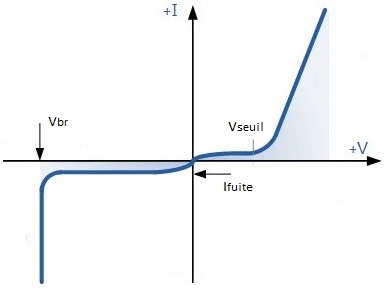
\includegraphics[width=0.70\textwidth]{images/reponse-theorique-diode}
    \caption{Courbe théorique des régions directe et inverse d'une diode.}
    \label{fig:reponse-theorique-diode}
\end{figure}

Modèle SPICE de la diode transil SLD8S33A :

\begin{lstlisting}
*define the model of the TVS SLD8S33A
*with Vbr=40.6
.model SLD8S33A D(Ron=.096 Roff=16.5Meg Vfwd=.7 Vrev=40.5 epsilon=1 revepsilon=0.4 mfg=Littlefuse type=TVS)
\end{lstlisting}


Pour le modèle ci-dessus, le circuit pour généré la réponse de cette diode, et sa réponse transitoire, sont illustrées sur les deux figures suivantes, fig. \ref{fig:circuit-courbe-transil} et fig. \ref{fig:reponse-diode-transil}.

\begin{figure}[H]
    \centering
    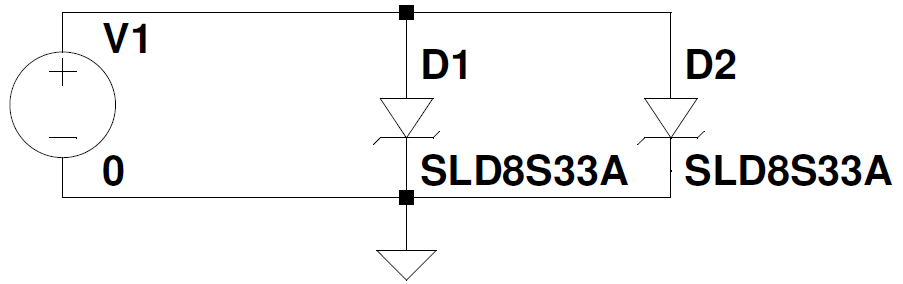
\includegraphics[width=0.80\textwidth]{images/circuit-courbe-transil}
    \caption{Circuit pour générer la réponse temporelle des deux diodes transil en parallèle.}
    \label{fig:circuit-courbe-transil}
\end{figure}

\begin{figure}[H]
    \centering
    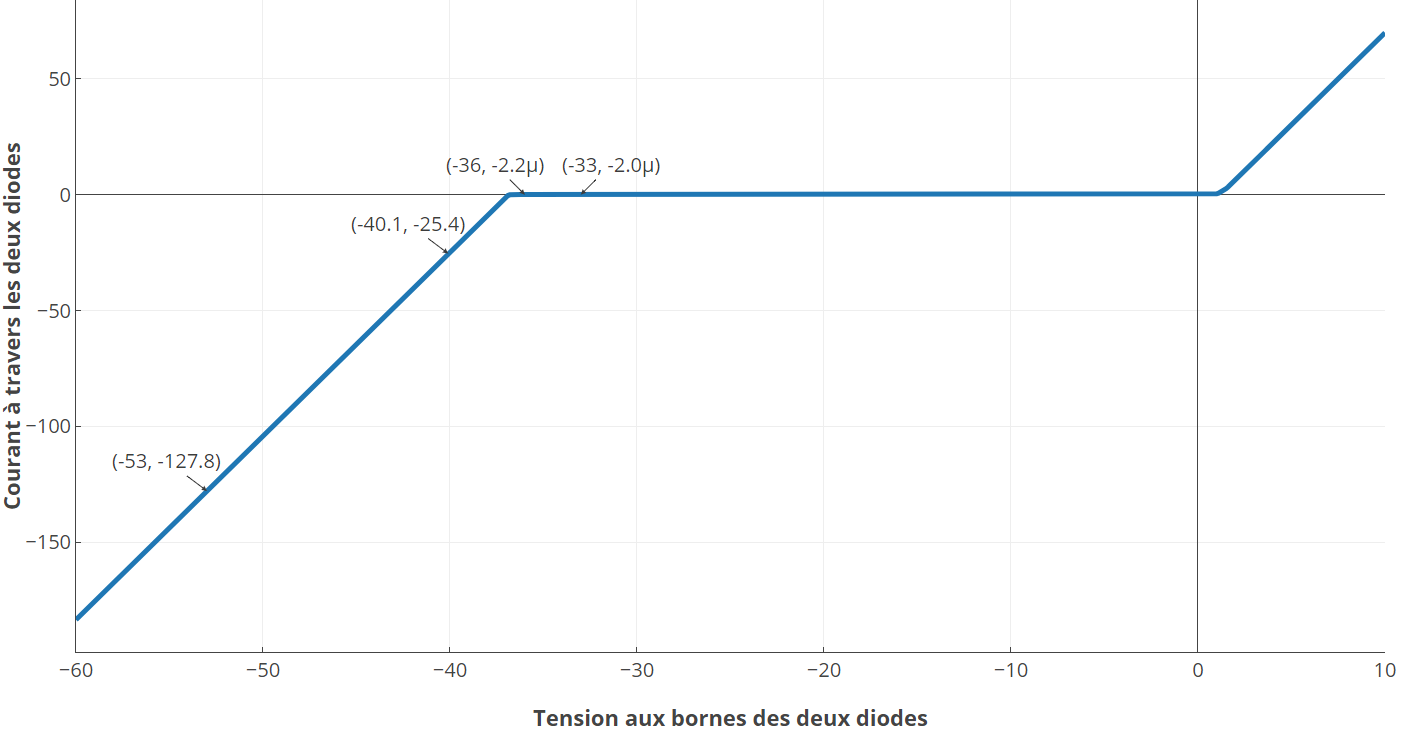
\includegraphics[width=1.00\textwidth]{images/reponse-diode-transil}
    \caption{Réponse temporelle des deux diodes transil en parallèle.}
    \label{fig:reponse-diode-transil}
\end{figure}

Le circuit écrêteur avec ce type de diode est illustré sur la figure \ref{fig:regulateur-transil} ; sa réponse est sur la figure \ref{fig:reponse-ecreteur-transil}.

\begin{figure}[H]
    \centering
    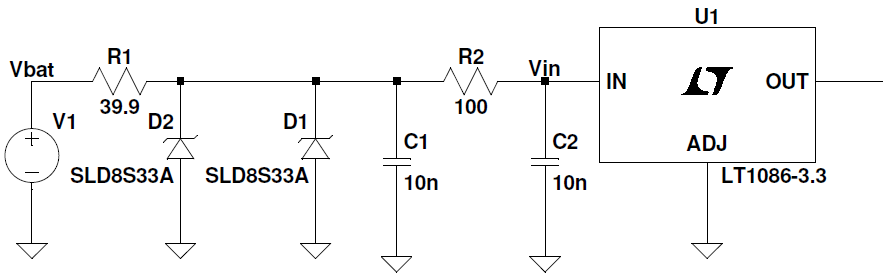
\includegraphics[width=1.00\textwidth]{images/regulateur-transil}
    \caption{Schéma du circuit écrêteur avec deux diodes transil.}
    \label{fig:regulateur-transil}
\end{figure}

\begin{figure}[H]
    \centering
    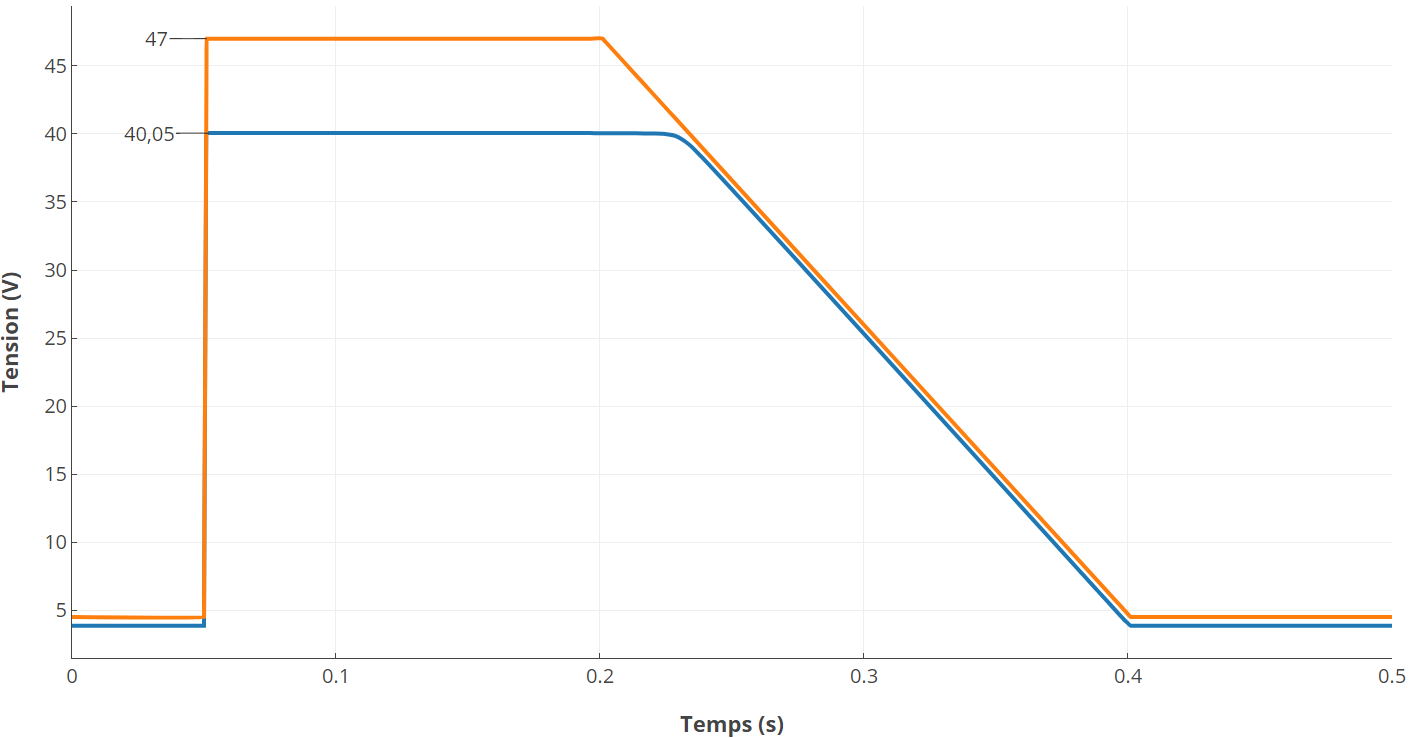
\includegraphics[width=1.00\textwidth]{images/reponse-ecreteur-transil}
    \caption{Tension $V_{BAT}$ (en orange) et la tension écrêté (en bleu).}
    \label{fig:reponse-ecreteur-transil}
\end{figure}



\subsection{Circuits avec des transistors}

L'autre option a été concevoir un circuit écrêteur avec des transistors et diodes zeners. Après avoir fait des simulations de quelques options, le meilleur circuit est montré sur la figure \ref{fig:ecreteur-avec-transistor} et sa réponse temporelle sur la figure \ref{fig:reponse-ecreteur-avec-transistor}.

\begin{figure}[H]
    \centering
    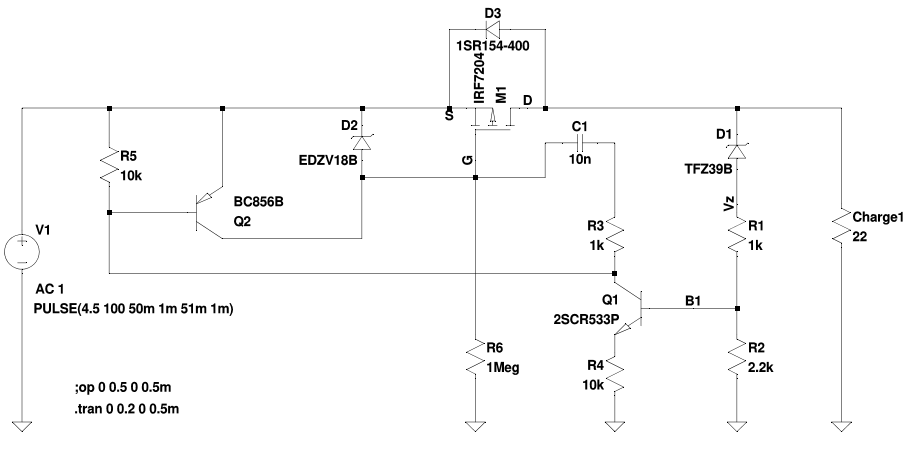
\includegraphics[width=1.00\textwidth]{images/ecreteur-avec-transistor}
    \caption{Schéma du circuit écrêteur avec des transistors et diodes zeners.}
    \label{fig:ecreteur-avec-transistor}
\end{figure}

\begin{figure}[H]
    \centering
    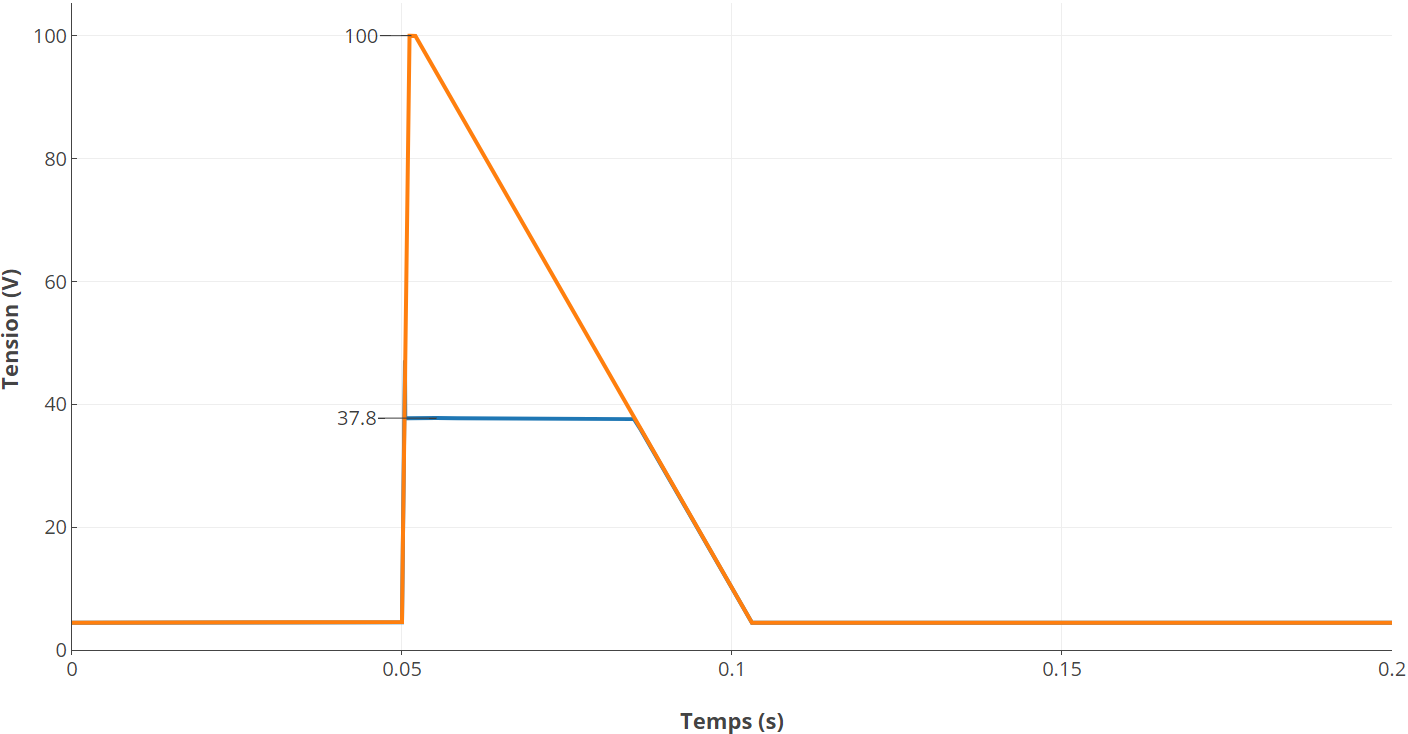
\includegraphics[width=1.00\textwidth]{images/reponse-ecreteur-avec-transistor}
    \caption{Tension $V_{BAT}$ (en orange) et la tension écrêté (en bleu).}
    \label{fig:reponse-ecreteur-avec-transistor}
\end{figure}




%\section{Entrée de fréquence FQ\_10}

%Não sei se essa seção vai ficar (não acho que fiz nada nisso)


\section{Commande d'un convertisseur DC-DC "buck"}

\textsc{Prendre des photos du convertisseur DC-DC et de la dernière carte que j'ai fait.}

\subsection{Version I}

On utilise le module TPS61086, qui est un buck, pour obtenir 3,3V de tension en sortie.

\begin{figure}[H]
    \centering
    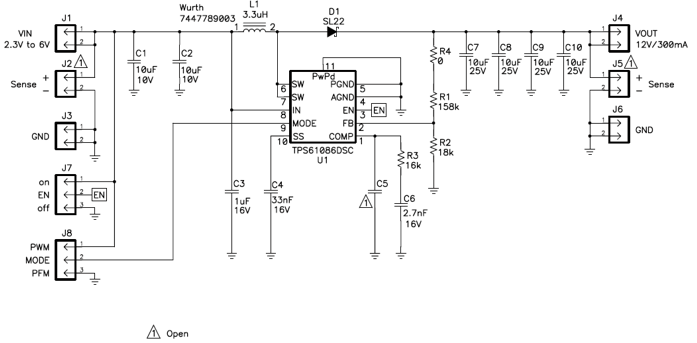
\includegraphics[width=1.00\textwidth]{images/schematic_TPS61086}
    \caption{Schéma de la carte du buck.}
    \label{fig:schematic_TPS61086}
\end{figure}


Nous allons changer le « feedback », comme montre la figure suivante :

\begin{figure}[H]
    \centering
    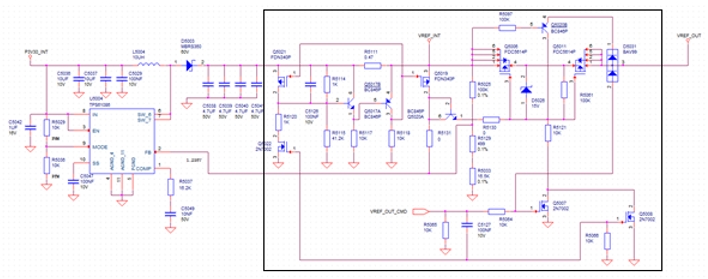
\includegraphics[width=1.00\textwidth]{images/circuit-contre-reaction-buck-v1}
    \caption{Circuit de contre-réaction et de protection pour le buck.}
    \label{fig:circuit-contre-reaction-buck-v1}
\end{figure}

J'ai monté la maquette du circuit encadré sur la figure ci-dessus. Le soudage a été difficile à cause de la taille de certains composants. Tous les composants sont du type SMD (surface mounted device). Par exemple, les deux transistors BC846P (PMOS and NMOS) a été très difficile à souder, une fois qu'il a fallu élever une patte pour qu'un court-circuit ne soit pas faite.


\begin{figure}[H]
    \centering
    \begin{subfigure}[t]{0.45\textwidth}
        \centering
        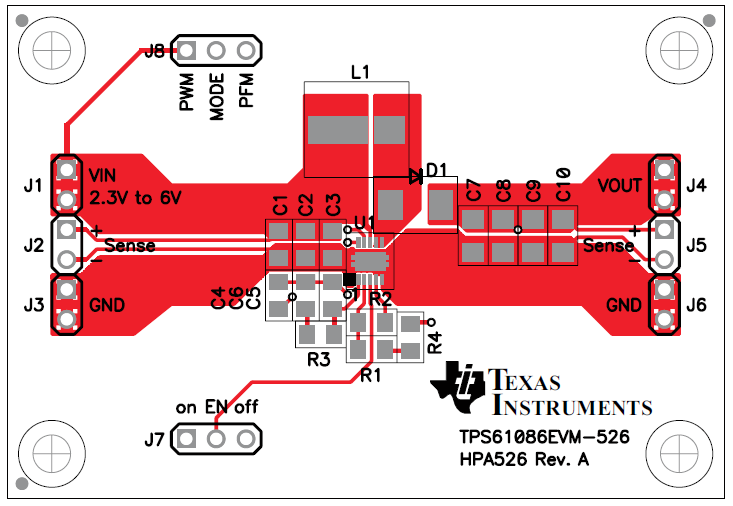
\includegraphics[width=0.90\textwidth]{images/carte-buck}
        \caption{Carte du module buck.}
    \end{subfigure}%
    ~ 
    \begin{subfigure}[t]{0.45\textwidth}
        \centering
        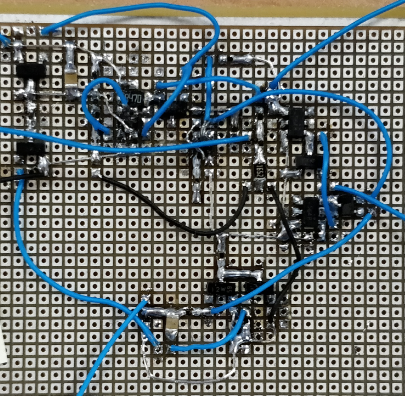
\includegraphics[width=0.90\textwidth]{images/carte-contre-reaction-buck-v1}
        \caption{Prototype de la carte électronique du circuit de contre-réaction pour le buck.}
    \end{subfigure}
    \caption{Convertisseur DC-DC buck et son circuit de contre-réaction.}
\end{figure}


\subsection{Version II}

Suite à divers tests avec le premier prototype, le schéma a été changé, voir la figure  pour le schéma de la version 2.

\begin{figure}[H]
    \centering
    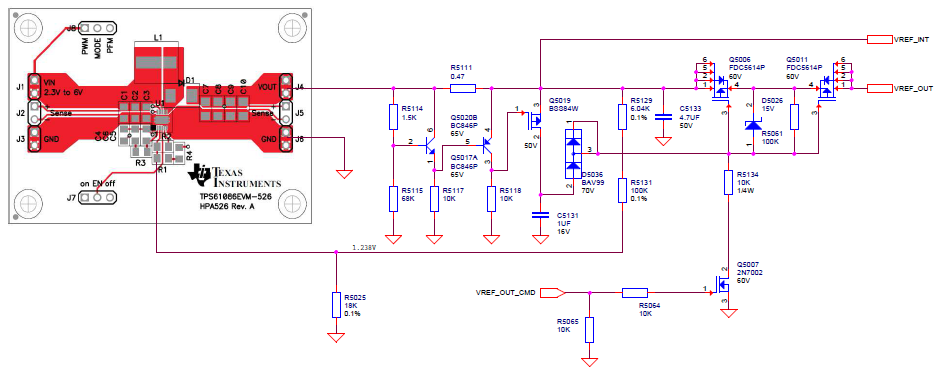
\includegraphics[width=1.00\textwidth]{images/circuit-contre-reaction-buck-v2}
    \caption{Deuxième prototype de la carte électronique du circuit de contre-réaction pour le buck.}
    \label{fig:circuit-contre-reaction-buck-v2}
\end{figure}


J'ai câblé le nouveau circuit de contre-réaction et le câblage sur une carte de prototypage est illustré sur la figure . 


\textsc{Prendre une photo de la dernière carte de la contre-réaction pour le buck.}


%\section{Carte d'interface JTAG}

% \textsc{Prendre des photos de la carte JTAG et des câbles que j'ai fait.}

% eu so fiz os cabos, acho que não vou colocar essa seção.


\section{Câblage d'une manipulation pour la qualification de la carte A-model}

La carte A-model est montrée sur la figure 




Le schéma de la manipulation pour des tests de qualification logicielle de l'UCM Nano A-model. Le schéma de cette manipulation est illustrée sur la figure \ref{fig:schema-manip-helene}.

\begin{figure}[H]
    \centering
    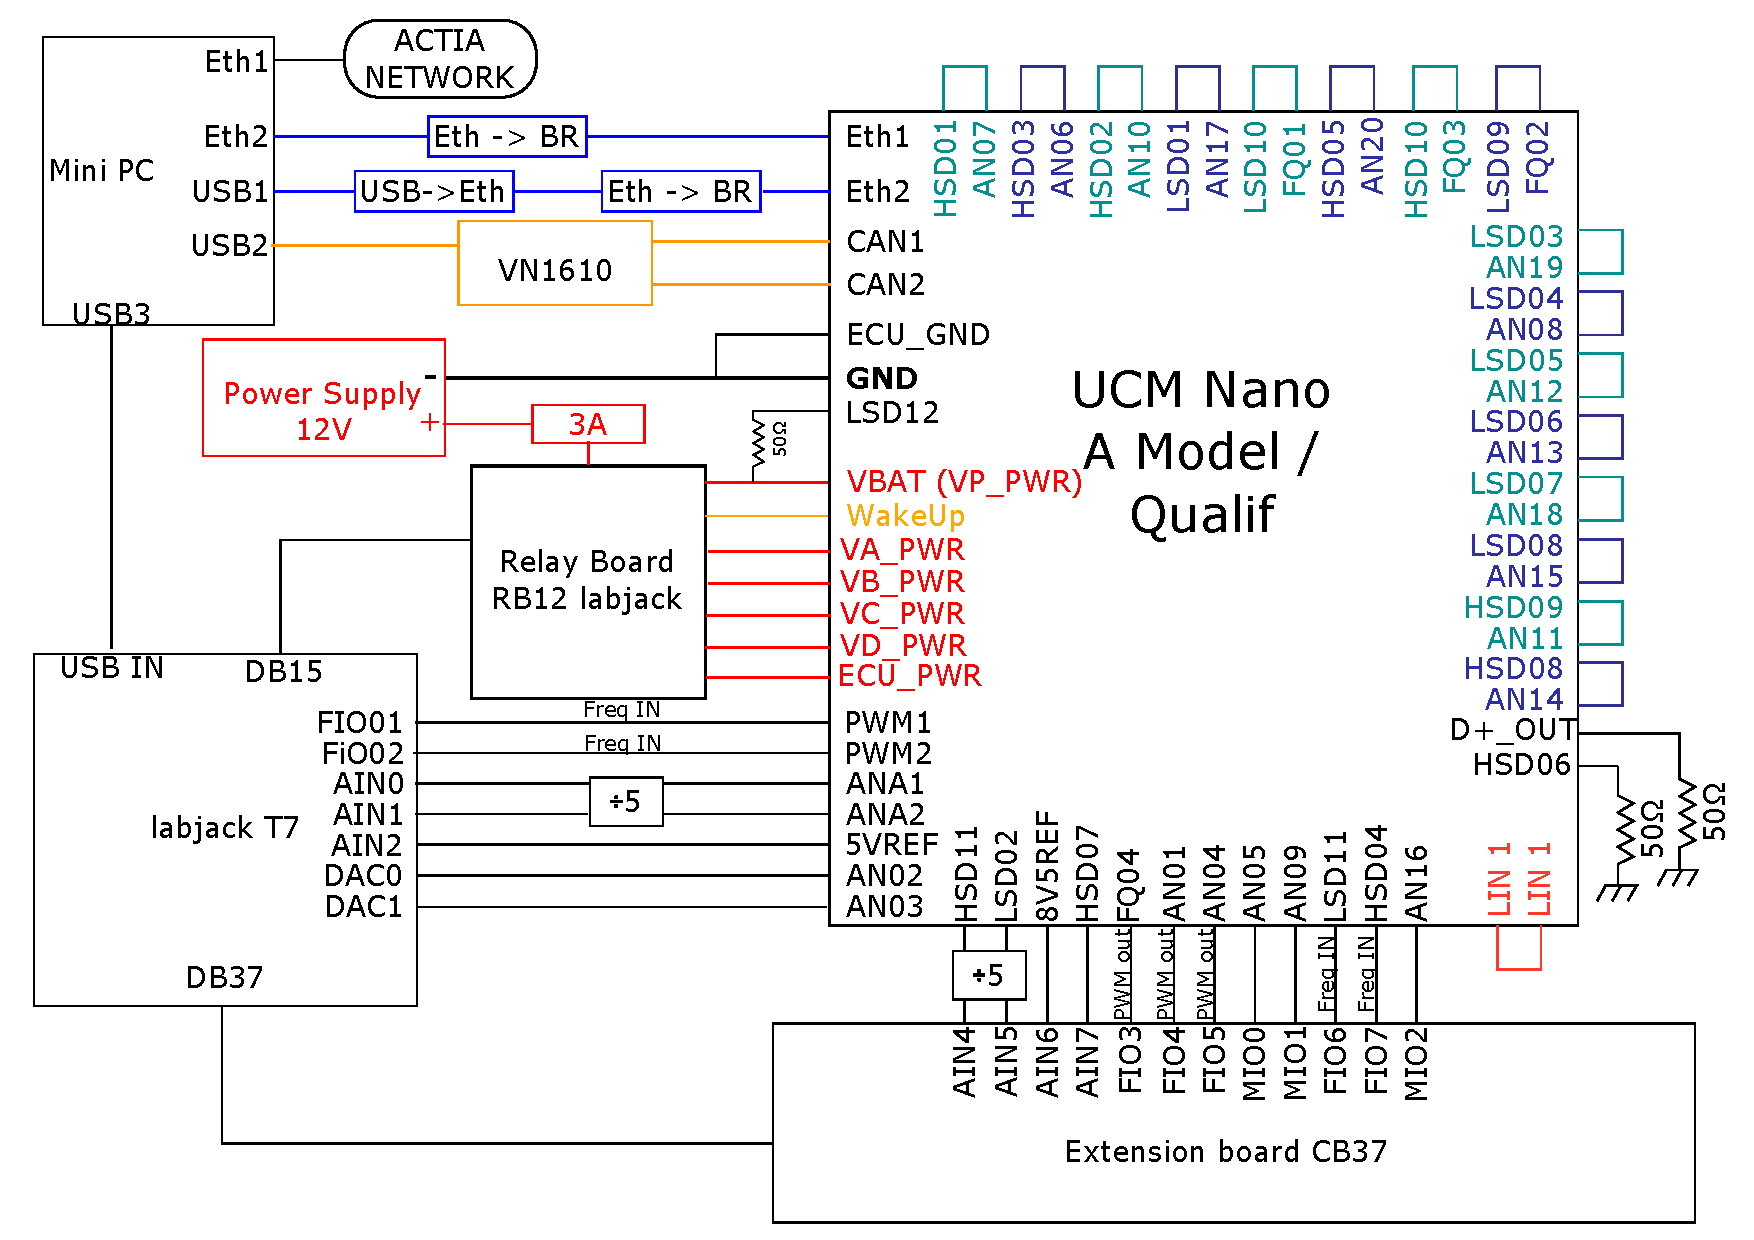
\includegraphics[width=1.00\textwidth]{images/schema-manip-helene}
    \caption{Schéma de la manipulation pour des tests du A-model.}
    \label{fig:schema-manip-helene}
\end{figure}


% \textsc{Prendre des photos de la manip que j'ai câblé pour Hellène.}


\section{Actualisation de la valise de test pour la carte B-model}



\begin{figure}[H]
    \centering
    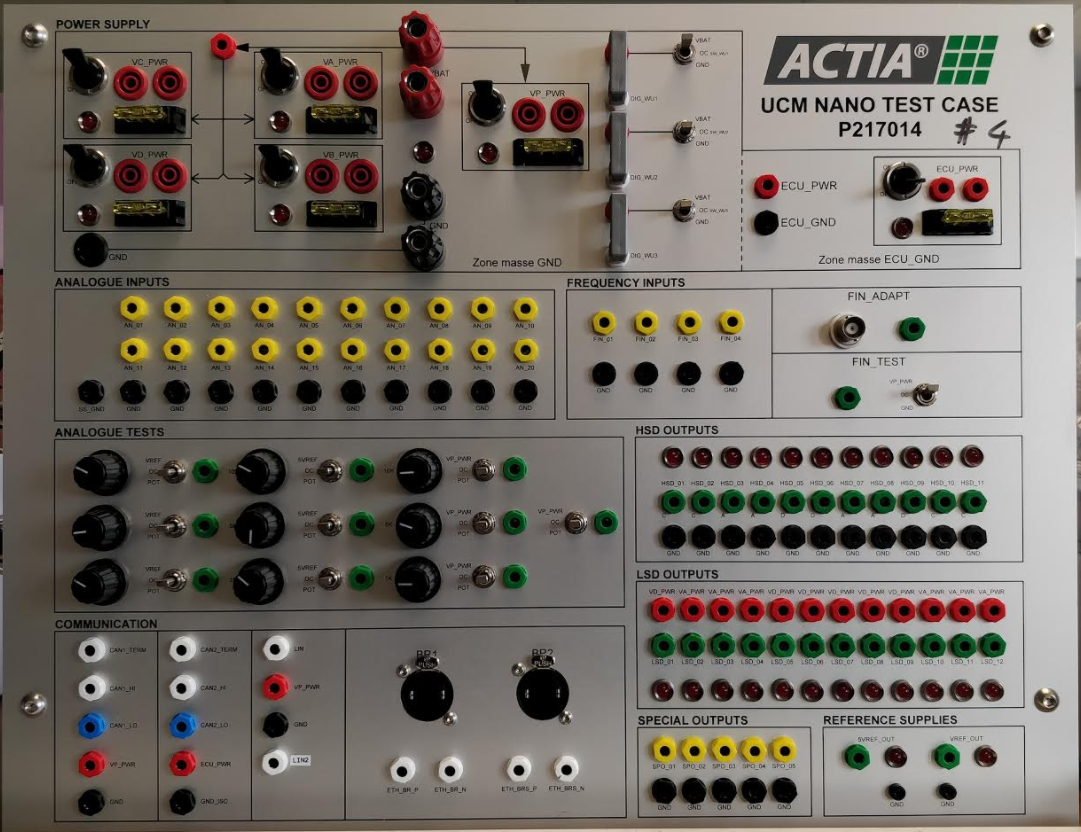
\includegraphics[width=1.00\textwidth]{images/valise-B_model}
    \caption{Valise de test du B-model.}
    \label{fig:valise-B_model}
\end{figure}

